\documentclass[aspectratio=169,10pt,xcolor={table,dvipsnames}]{beamer}

% ============================================================
% PACKAGES
% ============================================================
\usepackage[utf8]{inputenc}
\usepackage[T1]{fontenc}
\usepackage{lmodern}
\usepackage{graphicx}
\usepackage{amsmath,amssymb}
\usepackage{array}
\usepackage{tcolorbox}
\tcbuselibrary{skins}
\usepackage{tikz}
\usetikzlibrary{arrows.meta,positioning,calc,shapes.geometric}

% ============================================================
% MINIMALIST IEEE ACADEMIC PALETTE (Single Navy/Slate Family)
% ============================================================
\definecolor{Navy}{RGB}{11,37,69}           % Primary Deep Navy
\definecolor{SlateBlue}{RGB}{28,64,110}     % Professional Slate Blue Accent
\definecolor{Charcoal}{RGB}{30,41,59}       % High-Contrast Body Text
\definecolor{LightSilver}{RGB}{246,248,251} % Clean Card Background
\definecolor{BorderColor}{RGB}{205,215,226} % Subtle Card Border

\hypersetup{colorlinks=true,linkcolor=Navy,urlcolor=SlateBlue,citecolor=Navy}

% ============================================================
% BEAMER BASE THEME & SETTINGS (Light, Clean, High-Contrast)
% ============================================================
\setbeamercolor{background canvas}{bg=white}
\setbeamercolor{normal text}{fg=Charcoal}
\setbeamercolor{frametitle}{fg=Navy,bg=white}
\setbeamercolor{itemize item}{fg=SlateBlue}
\setbeamercolor{itemize subitem}{fg=SlateBlue}
\setbeamertemplate{navigation symbols}{}
\setbeamertemplate{headline}{}
\setbeamertemplate{itemize item}{\small$\blacktriangleright$}
\setbeamertemplate{itemize subitem}{\scriptsize$\circ$}

% Clean, Minimalist Frametitle (Crisp White Background, Navy Title & Subtle Divider)
\setbeamertemplate{frametitle}{%
  \nointerlineskip
  \begin{beamercolorbox}[wd=\paperwidth,ht=3.0ex,dp=1.0ex,leftskip=0.8cm,rightskip=0.8cm]{frametitle}
    {\fontsize{11}{13}\selectfont\bfseries\color{Navy}\insertframetitle}%
    \hfill{\fontsize{7.5}{9}\selectfont\color{Charcoal!60}\insertframenumber\,/\,\inserttotalframenumber}
  \end{beamercolorbox}%
  \vspace{-2pt}%
  {\color{BorderColor}\hrule height 0.8pt}%
  \vspace{0.14cm}%
}
\setbeamertemplate{footline}{}

% ============================================================
% STANDARDIZED ACADEMIC CARDS (Light Backgrounds, Subtle Borders)
% ============================================================
\tcbset{
  academiccard/.style={
    enhanced,arc=2.5pt,boxrule=0.7pt,
    left=6pt,right=6pt,top=3.5pt,bottom=3.5pt,
    fonttitle=\bfseries\scriptsize,
    colback=LightSilver,colframe=BorderColor,
    coltitle=Navy
  },
  modcard/.style={
    enhanced,arc=2pt,boxrule=0.6pt,
    left=5pt,right=5pt,top=3pt,bottom=3pt,
    fonttitle=\bfseries\scriptsize,
    colback=LightSilver,colframe=BorderColor,
    coltitle=Navy
  }
}
\newtcolorbox{navytitlecard}[1]{academiccard,colframe=BorderColor,coltitle=Navy,title={#1}}
\newtcolorbox{plaincard}[1]{academiccard,colframe=BorderColor,coltitle=Navy,title={#1}}

% ============================================================
\begin{document}
% ============================================================

% ------------------------------------------------------------
% SLIDE 1 — TITLE SLIDE (Official Banner + Centered Title + Pillars)
% ------------------------------------------------------------
\begin{frame}[t,plain]
  % 1. Official College Header Banner (Compact & Proportionally Scaled)
  \vspace*{0.15cm}
  \centerline{
\includegraphics[width=10.8cm,height=1.85cm,keepaspectratio]{college_header.png}}
  \vspace{0.08cm}
  \centerline{\color{BorderColor}\rule{10.8cm}{0.8pt}}

  \vspace{0.25cm}

  % 2. Project Title Box
  \begin{tcolorbox}[
    enhanced,colback=LightSilver,colframe=BorderColor,
    arc=3pt,boxrule=0.8pt,
    left=12pt,right=12pt,top=8pt,bottom=8pt]
    \centering
    {\fontsize{12.5}{16.5}\selectfont\bfseries\color{Navy}%
      An Evidence-Driven Framework for Continuous\\[3pt]
      Programming Competency Development\\[3pt]
      through Collaborative Learning}
  \end{tcolorbox}

  \vspace{0.22cm}

  % 3. Core Research Pillars (Balanced Lower Slide Layout)
  \begin{columns}[T]
    \begin{column}{0.315\textwidth}
      \begin{tcolorbox}[academiccard,title={Collaborative Learning}]
        \fontsize{6.2}{7.5}\selectfont
        Synchronous peer study circles, pair programming, and collaborative walkthroughs.
      \end{tcolorbox}
    \end{column}

    \begin{column}{0.315\textwidth}
      \begin{tcolorbox}[academiccard,title={Continuous Telemetry}]
        \fontsize{6.2}{7.5}\selectfont
        Multi-source ingestion from live IDE logs, GitHub commits, and micro-tasks.
      \end{tcolorbox}
    \end{column}

    \begin{column}{0.315\textwidth}
      \begin{tcolorbox}[academiccard,title={Closed-Loop Evaluation}]
        \fontsize{6.2}{7.5}\selectfont
        Dynamic deficit diagnosis, targeted remediation, and empirical skill gain ($g$).
      \end{tcolorbox}
    \end{column}
  \end{columns}

  % 4. Bottom Accent Rule
  \vfill
  \centerline{\color{BorderColor}\rule{10.8cm}{0.8pt}}
\end{frame}

% ------------------------------------------------------------
% SLIDE 2 — INTRODUCTION
% ------------------------------------------------------------
\begin{frame}[t]{Introduction}
  \begin{columns}[T]
    \begin{column}{0.485\textwidth}
      \begin{navytitlecard}{1.\;Continuous Programming Practice}
        \fontsize{6.5}{7.8}\selectfont
        \begin{itemize}\setlength{\itemsep}{1pt}
          \item Programming competency is an accretive, empirical skill developed through sustained coding and iterative problem-solving.
          \item Algorithmic thinking, syntax mastery, and debugging cannot be mastered through passive classroom instruction alone.
        \end{itemize}
      \end{navytitlecard}
      \vspace{0.08cm}
      \begin{plaincard}{2.\;Limitations of Traditional Assessment}
        \fontsize{6.5}{7.8}\selectfont
        \begin{itemize}\setlength{\itemsep}{1pt}
          \item Periodic terminal examinations offer only an episodic snapshot of student performance under test-taking pressure.
          \item Memorization under examination stress fails to reflect sustained analytical capability or industry-readiness.
        \end{itemize}
      \end{plaincard}
    \end{column}

    \begin{column}{0.485\textwidth}
      \begin{navytitlecard}{3.\;Distributed Learning Evidence}
        \fontsize{6.5}{7.8}\selectfont
        \begin{itemize}\setlength{\itemsep}{1pt}
          \item Students generate meaningful evidence across GitHub, LeetCode, coding sandboxes, and collaborative peer sessions.
          \item These signals remain scattered across disconnected silos and are rarely integrated into academic evaluation.
        \end{itemize}
      \end{navytitlecard}
      \vspace{0.08cm}
      \begin{plaincard}{4.\;Need for Continuous Competency Development}
        \fontsize{6.5}{7.8}\selectfont
        \begin{itemize}\setlength{\itemsep}{1pt}
          \item Learners need immediate diagnostic feedback, peer-guided interventions, and structured reassessment cycles.
          \item Bridges deficit identification with verifiable longitudinal skill progression over time.
        \end{itemize}
      \end{plaincard}
    \end{column}
  \end{columns}

  \vspace{0.10cm}
  \begin{tcolorbox}[
    enhanced,colback=LightSilver,colframe=BorderColor,
    arc=2pt,boxrule=0.6pt,
    left=6pt,right=6pt,top=2.5pt,bottom=2.5pt]
    \centering\fontsize{6.5}{7.8}\selectfont
    \textbf{\color{Navy}Research Imperative:}\;Transitioning computing education from sporadic summative exams to a continuous telemetry-driven model that unifies daily coding practice with structured collaborative peer interventions.
  \end{tcolorbox}
\end{frame}

% ------------------------------------------------------------
% SLIDE 3 — ABSTRACT: PROBLEM & RESEARCH OBJECTIVE
% ------------------------------------------------------------
\begin{frame}[t]{Abstract\enspace---\enspace Problem \& Research Objective}
  \begin{tcolorbox}[
    enhanced,colback=LightSilver,colframe=BorderColor,
    arc=2.5pt,boxrule=0.7pt,
    left=8pt,right=8pt,top=4pt,bottom=4pt]
    \fontsize{7.2}{8.8}\selectfont
    \textbf{\color{Navy}The Core Problem:}\quad
    Current programming pedagogy suffers from three critical disconnects:
    \vspace{2pt}
    \begin{itemize}\setlength{\itemsep}{1.5pt}
      \item \textbf{Fragmented Evidence:}\;Coding activity across GitHub, LeetCode, and labs remains unaggregated.
      \item \textbf{Isolated Collaboration:}\;Peer learning occurs informally without telemetry or diagnostic capture.
      \item \textbf{Absence of Closed Loop:}\;Summative grades fail to trigger targeted remedial problem sets or reassessment.
    \end{itemize}
  \end{tcolorbox}

  \vspace{0.10cm}

  \begin{tcolorbox}[
    enhanced,colback=LightSilver,colframe=BorderColor,
    arc=2.5pt,boxrule=0.7pt,
    left=8pt,right=8pt,top=4pt,bottom=4pt]
    \fontsize{7.2}{8.8}\selectfont
    \textbf{\color{Navy}Research Objective:}\quad
    To design, implement, and evaluate an evidence-driven framework that integrates collaborative peer learning, continuous assessment, and multi-source telemetry into a \textbf{measurable, closed-loop longitudinal competency development cycle}.
    \vspace{2pt}
    \begin{itemize}\setlength{\itemsep}{1.5pt}
      \item \textbf{Target 1:}\;Ingest real-time coding telemetry from live IDE sessions and external repository webhooks.
      \item \textbf{Target 2:}\;Map student skills dynamically against IEEE/ACM CS Curricula 2023 competency rubrics.
      \item \textbf{Target 3:}\;Deliver automated peer-matched interventions and measure verified learning gains ($g$).
    \end{itemize}
  \end{tcolorbox}

  \vspace{0.10cm}

  \begin{tcolorbox}[
    enhanced,colback=LightSilver,colframe=BorderColor,
    arc=2.5pt,boxrule=0.7pt,
    left=8pt,right=8pt,top=4pt,bottom=4pt]
    \centering\fontsize{7.2}{8.8}\selectfont
    \textbf{\color{Navy}Core Evaluative Research Question:}\\[2pt]
    \textit{``Can collaborative peer learning combined with continuous assessment and multi-source evidence \textbf{measurably improve and reliably track} student programming competency over time?''}
  \end{tcolorbox}
\end{frame}

% ------------------------------------------------------------
% SLIDE 4 — ABSTRACT: PROPOSED RESEARCH CYCLE
% ------------------------------------------------------------
\begin{frame}[t]{Abstract\enspace---\enspace Proposed Research Cycle}
  \centering
  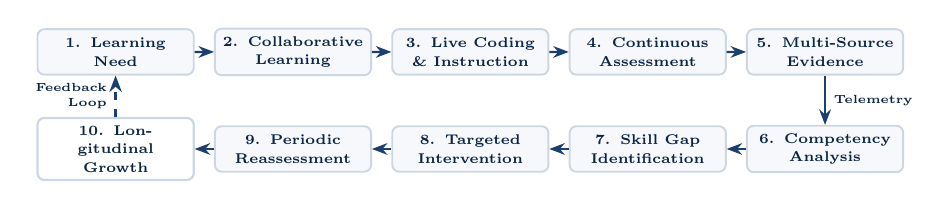
\begin{tikzpicture}[
      scale=0.85,every node/.style={transform shape},
      bNode/.style={draw=BorderColor,fill=LightSilver,rounded corners=2.5pt,
                    minimum width=2.30cm,minimum height=0.68cm,text width=2.10cm,
                    font=\fontsize{6.5}{7.8}\selectfont\bfseries,align=center,text=Navy,line width=0.7pt},
      tNode/.style={draw=BorderColor,fill=LightSilver,rounded corners=2.5pt,
                    minimum width=2.30cm,minimum height=0.68cm,text width=2.10cm,
                    font=\fontsize{6.5}{7.8}\selectfont\bfseries,align=center,text=Navy,line width=0.7pt},
      fNode/.style={draw=BorderColor,fill=white,rounded corners=2.5pt,
                    minimum width=2.30cm,minimum height=0.68cm,text width=2.10cm,
                    font=\fontsize{6.5}{7.8}\selectfont\bfseries,align=center,text=Navy,line width=0.8pt},
      ar/.style={-{Stealth[scale=0.85]},line width=0.8pt,color=SlateBlue}
    ]

    % Row 1: Evidence Ingestion (Left to Right)
    \node(n1)[bNode] at (0, 1.45) {1. Learning\\Need};
    \node(n2)[bNode] at (2.65, 1.45) {2. Collaborative\\Learning};
    \node(n3)[bNode] at (5.30, 1.45) {3. Live Coding\\\& Instruction};
    \node(n4)[bNode] at (7.95, 1.45) {4. Continuous\\Assessment};
    \node(n5)[bNode] at (10.60, 1.45) {5. Multi-Source\\Evidence};

    % Row 2: Diagnostic & Closed Loop (Right to Left)
    \node(n6)[tNode] at (10.60, 0) {6. Competency\\Analysis};
    \node(n7)[tNode] at (7.95, 0) {7. Skill Gap\\Identification};
    \node(n8)[tNode] at (5.30, 0) {8. Targeted\\Intervention};
    \node(n9)[tNode] at (2.65, 0) {9. Periodic\\Reassessment};
    \node(n10)[fNode] at (0, 0) {10. Longitudinal\\Growth};

    % Phase 1 Arrows
    \draw[ar] (n1) -- (n2);
    \draw[ar] (n2) -- (n3);
    \draw[ar] (n3) -- (n4);
    \draw[ar] (n4) -- (n5);

    % Transition Downward Arrow on Right
    \draw[ar] (n5.south) -- node[right,font=\fontsize{5.5}{6.5}\selectfont\bfseries,color=Navy]{Telemetry} (n6.north);

    % Phase 2 Arrows
    \draw[ar] (n6) -- (n7);
    \draw[ar] (n7) -- (n8);
    \draw[ar] (n8) -- (n9);
    \draw[ar] (n9) -- (n10);

    % Vertical Closed-Loop Feedback Arrow on Left (Clean & Unobstructed)
    \draw[ar,dashed,line width=0.9pt] (n10.north) -- 
      node[left,font=\fontsize{5.5}{6.5}\selectfont\bfseries,color=Navy,align=right]%
      {Feedback\\Loop} (n1.south);
  \end{tikzpicture}

  \vspace{0.12cm}

  \begin{columns}[T]
    \begin{column}{0.485\textwidth}
      \begin{tcolorbox}[academiccard,title={Phase 1 : Interaction \& Telemetry (Nodes 1--5)}]
        \fontsize{6.5}{7.8}\selectfont
        Captures live collaborative coding interactions, syntax edits, execution traces, and external repository commits into a normalized telemetry stream.
      \end{tcolorbox}
    \end{column}
    \begin{column}{0.485\textwidth}
      \begin{tcolorbox}[academiccard,title={Phase 2 : Diagnosis \& Closed Loop (Nodes 6--10)}]
        \fontsize{6.5}{7.8}\selectfont
        Dynamically analyzes concept deficits, pairs students for targeted peer remediation, and empirically verifies longitudinal competency growth via reassessment.
      \end{tcolorbox}
    \end{column}
  \end{columns}

  \vspace{0.08cm}
  \begin{tcolorbox}[
    enhanced,colback=LightSilver,colframe=BorderColor,
    arc=2pt,boxrule=0.6pt,
    left=6pt,right=6pt,top=2.5pt,bottom=2.5pt]
    \centering\fontsize{6.5}{7.8}\selectfont
    \textbf{\color{Navy}Core Architectural Novelty:}\;The innovation lies in the \textbf{end-to-end integration and empirical evaluation of the complete closed-loop cycle} (Learning $\to$ Telemetry $\to$ Diagnosis $\to$ Intervention $\to$ Reassessment), rather than treating any element as an isolated feature.
  \end{tcolorbox}
\end{frame}

% ------------------------------------------------------------
% SLIDE 5 — LITERATURE SURVEY (Clean IEEE Monochrome Table)
% ------------------------------------------------------------
\begin{frame}[t]{Literature Survey}
  \vspace{-0.1cm}
  \centering
  {\fontsize{6.0}{7.4}\selectfont
  \renewcommand{\arraystretch}{1.12}
  \begin{tabular}{|c|p{3.8cm}|p{2.3cm}|c|p{4.7cm}|}
    \hline
    \rowcolor{LightSilver}
    \textbf{S.No} & \textbf{Paper Title} & \textbf{Author(s)} & \textbf{Year} & \textbf{Drawbacks \& Research Limitations}\\
    \hline
    \textbf{1} &
    \textbf{Shaking The Silos: Impact of Sequential Live Coding on Students' Performance} &
    Cho K.; Ali S.F.; Bang S.J.; Anwar S. & 2024 &
    Investigates live coding as an isolated teaching technique; lacks multi-source evidence tracking and automated remediation.\\
    \hline
    \rowcolor{LightSilver}
    \textbf{2} &
    \textbf{Engaging Minds: Impact of Sequential Live Coding on Academic Engagement} &
    Cho K.; Ali S.F.; Bang S.J.; Anwar S. & 2025 &
    Evaluates behavioral engagement only; does not link collaborative evidence with longitudinal reassessment or skill growth.\\
    \hline
    \textbf{3} &
    \textbf{Integration of Multiple Sources to Anticipate Student Performance Using Learning Analytics} &
    Moreno-Marcos P.M.\ et al.\ (IEEE ICALT) & 2025 &
    Demonstrates predictive modeling but lacks active collaborative intervention and closed-loop remedial practice cycles.\\
    \hline
    \rowcolor{LightSilver}
    \textbf{4} &
    \textbf{A Pragmatic Framework for Assessing Learning Outcomes in Competency-Based Courses} &
    Vargas H.\ et al.\ (IEEE Trans.\ Educ.) & 2024 &
    Defines static competency mapping; lacks real-time peer coding telemetry and adaptive feedback mechanisms.\\
    \hline
    \textbf{5} &
    \textbf{Development and Classroom Evaluation of a Static-Assessment Programming Practice Platform} &
    Jeon J.\ et al.\ (IEEE Access) & 2026 &
    Confined to static automated grading; does not support collaborative peer learning or longitudinal tracking.\\
    \hline
  \end{tabular}}

  \vspace{0.10cm}
  \begin{tcolorbox}[
    enhanced,colback=LightSilver,colframe=BorderColor,
    arc=2pt,boxrule=0.7pt,
    left=6pt,right=6pt,top=3pt,bottom=3pt]
    \centering\fontsize{6.5}{7.8}\selectfont
    \textbf{\color{Navy}Identified Research Gap:}\;Existing studies examine live coding, peer collaboration, and learning analytics as \textbf{disconnected silos}. No established framework integrates them into an \textbf{adaptive, closed-loop longitudinal competency development and empirical validation system}.
  \end{tcolorbox}
\end{frame}

% ------------------------------------------------------------
% SLIDE 6 — EXISTING SYSTEM & DRAWBACKS
% ------------------------------------------------------------
\begin{frame}[t]{Existing System\enspace---\enspace Drawbacks}
  \begin{columns}[T]
    % Left Column: Conventional Flowchart
    \begin{column}{0.43\textwidth}
      \begin{navytitlecard}{Conventional Fragmented Flow}
        \centering\vspace{1pt}
        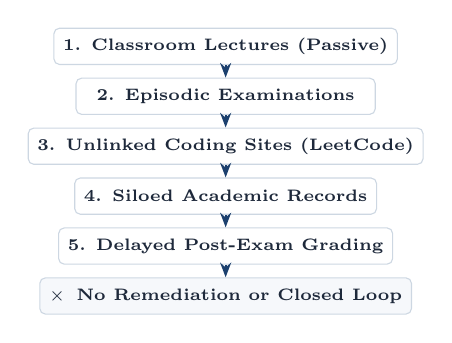
\begin{tikzpicture}[
          node distance=0.16cm,
          bk/.style={draw=BorderColor,fill=white,rounded corners=2pt,
                     minimum width=3.8cm,minimum height=0.46cm,
                     font=\fontsize{6.2}{7.5}\selectfont\bfseries,text=Charcoal},
          ar/.style={-{Stealth[scale=0.8]},thick,SlateBlue}
        ]
          \node(e1)[bk]{1. Classroom Lectures (Passive)};
          \node(e2)[bk,below=of e1]{2. Episodic Examinations};
          \node(e3)[bk,below=of e2]{3. Unlinked Coding Sites (LeetCode)};
          \node(e4)[bk,below=of e3]{4. Siloed Academic Records};
          \node(e5)[bk,below=of e4]{5. Delayed Post-Exam Grading};
          \node(e6)[bk,below=of e5,draw=BorderColor,fill=LightSilver,text=Charcoal]{$\times$\enspace No Remediation or Closed Loop};

          \draw[ar] (e1) -- (e2);
          \draw[ar] (e2) -- (e3);
          \draw[ar] (e3) -- (e4);
          \draw[ar] (e4) -- (e5);
          \draw[ar,SlateBlue,dashed] (e5) -- (e6);
        \end{tikzpicture}
      \end{navytitlecard}
    \end{column}

    % Right Column: Drawbacks
    \begin{column}{0.55\textwidth}
      \begin{plaincard}{Systemic Drawbacks}
        \fontsize{6.8}{8.2}\selectfont
        \begin{enumerate}\setlength{\itemsep}{2.2pt}
          \item \textbf{Scattered Evidence:}\;GitHub, LeetCode, and lab telemetry are never unified into a single competency profile.
          \item \textbf{Snapshot Bias:}\;Periodic tests evaluate memorization under stress rather than sustained problem-solving ability.
          \item \textbf{Isolated Peer Data:}\;Peer study sessions occur informally without tracking or diagnostic integration.
          \item \textbf{Delayed Intervention:}\;Deficits surface only after summative exams, preventing timely remediation.
          \item \textbf{Absence of Closed Loop:}\;No automated feedback connects identified gaps to adaptive practice sets.
          \item \textbf{Longitudinal Blindspot:}\;Institutional rubrics fail to measure or plot skill progression over time.
        \end{enumerate}
      \end{plaincard}
    \end{column}
  \end{columns}

  \vspace{0.12cm}
  \begin{tcolorbox}[
    enhanced,colback=LightSilver,colframe=BorderColor,
    arc=2pt,boxrule=0.6pt,
    left=6pt,right=6pt,top=2.5pt,bottom=2.5pt]
    \centering\fontsize{6.5}{7.8}\selectfont
    \textbf{\color{Navy}Critical Consequence:}\;Traditional linear teaching produces a permanent gap between student evaluation and skill remediation, leaving learners without actionable pathways to algorithmic mastery.
  \end{tcolorbox}
\end{frame}

% ------------------------------------------------------------
% SLIDE 7 — PROPOSED SYSTEM & ADVANTAGES
% ------------------------------------------------------------
\begin{frame}[t]{Proposed System\enspace---\enspace Advantages}
  \begin{columns}[T]
    % Left Column: Architecture Overview + Contribution
    \begin{column}{0.46\textwidth}
      \begin{navytitlecard}{Proposed Closed-Loop Model}
        \fontsize{6.8}{8.2}\selectfont
        \renewcommand{\arraystretch}{1.12}
        \begin{tabular}{@{}cl@{}}
          {\color{Navy}$\blacktriangleright$} & \textbf{Collaborative Peer Learning}\\
          {\color{Navy}$+$} & Live Synchronous Coding Walkthroughs\\
          {\color{Navy}$+$} & Continuous Micro-Assessments\\
          {\color{Navy}$+$} & Multi-Source Telemetry (GitHub/LeetCode)\\[2pt]
          \hline\\[-5pt]
          {\color{Navy}$\downarrow$} & \textbf{Competency Vector Scoring}\\
          {\color{Navy}$\downarrow$} & \textbf{Automated Skill Gap Detection}\\
          {\color{Navy}$\downarrow$} & \textbf{Targeted Peer Remediation}\\
          {\color{Navy}$\downarrow$} & \textbf{Isomorphic Reassessment}\\[2pt]
          \hline\\[-5pt]
          {\color{Navy}$\circlearrowleft$} & \textbf{Longitudinal Growth Tracking ($g$)}
        \end{tabular}
      \end{navytitlecard}
      \vspace{0.08cm}
      \begin{tcolorbox}[
        enhanced,colback=LightSilver,colframe=BorderColor,
        arc=2pt,boxrule=0.6pt,
        left=5pt,right=5pt,top=2.5pt,bottom=2.5pt]
        \fontsize{6.5}{7.8}\selectfont\color{Navy}
        \textbf{Core Contribution:}\;Transforms terminal testing into an \textbf{adaptive, closed-loop competency validation framework}.
      \end{tcolorbox}
    \end{column}

    % Right Column: Key Advantages
    \begin{column}{0.52\textwidth}
      \begin{plaincard}{Six Key Advantages}
        \fontsize{6.8}{8.2}\selectfont
        \begin{enumerate}\setlength{\itemsep}{2.2pt}
          \item \textbf{Unified Evidence Pipeline:}\;Ingests commits, problem submissions, and IDE logs centrally.
          \item \textbf{Collaborative Rubrics:}\;Converts peer coding interactions into measurable competency metrics.
          \item \textbf{Continuous Tracking:}\;Rolling skill estimation replaces biased episodic testing.
          \item \textbf{Precision Gap Detection:}\;Pinpoints concept-level algorithmic deficits automatically.
          \item \textbf{Adaptive Remediation:}\;Algorithmic peer-matching delivers targeted remedial problem sets.
          \item \textbf{Empirical Validation:}\;Reassessment measures actual normalized learning gain ($g$).
        \end{enumerate}
      \end{plaincard}
    \end{column}
  \end{columns}

  \vspace{0.12cm}
  \begin{tcolorbox}[
    enhanced,colback=LightSilver,colframe=BorderColor,
    arc=2pt,boxrule=0.6pt,
    left=6pt,right=6pt,top=2.5pt,bottom=2.5pt]
    \centering\fontsize{6.5}{7.8}\selectfont
    \textbf{\color{Navy}Educational Paradigm Shift:}\;Moves pedagogy from subjective inspection to \textbf{verifiable, telemetry-backed algorithmic competency progression}.
  \end{tcolorbox}
\end{frame}

% ------------------------------------------------------------
% SLIDE 8 — SYSTEM ARCHITECTURE & FLOW
% ------------------------------------------------------------
\begin{frame}[t]{System Architecture\enspace---\enspace Flow}
  \centering
  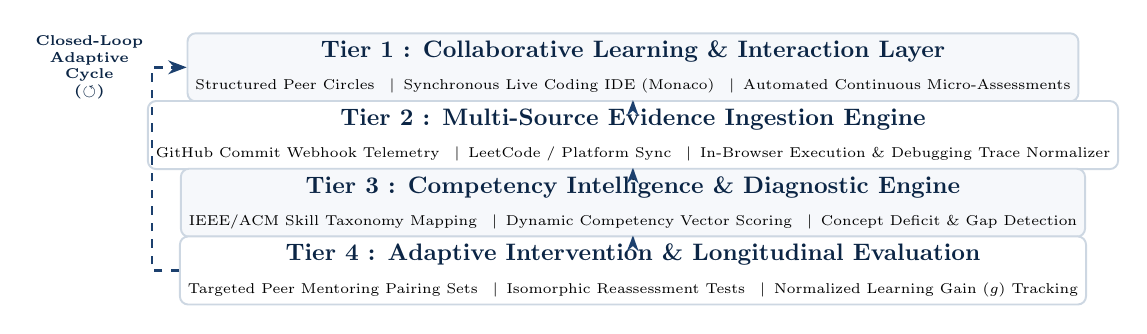
\begin{tikzpicture}[
      scale=0.86,every node/.style={transform shape},
      tierBox/.style={draw=BorderColor,fill=LightSilver,rounded corners=3pt,
                      minimum width=11.6cm,minimum height=0.74cm,
                      line width=0.7pt,align=center},
      arDown/.style={-{Stealth[scale=0.85]},thick,SlateBlue}
    ]

    % Tier 1: Collaborative Learning & Interaction Layer
    \node(t1)[tierBox] at (0, 1.95) {%
      \textbf{\color{Navy}Tier 1 : Collaborative Learning \& Interaction Layer}\\[1.5pt]
      \fontsize{6.2}{7.5}\selectfont
      Structured Peer Circles \enspace\textbar\enspace
      Synchronous Live Coding IDE (Monaco) \enspace\textbar\enspace
      Automated Continuous Micro-Assessments};

    % Tier 2: Multi-Source Evidence Ingestion Layer
    \node(t2)[tierBox,fill=white] at (0, 0.95) {%
      \textbf{\color{Navy}Tier 2 : Multi-Source Evidence Ingestion Engine}\\[1.5pt]
      \fontsize{6.2}{7.5}\selectfont
      GitHub Commit Webhook Telemetry \enspace\textbar\enspace
      LeetCode / Platform Sync \enspace\textbar\enspace
      In-Browser Execution \& Debugging Trace Normalizer};

    % Tier 3: Competency Intelligence & Analytics Engine
    \node(t3)[tierBox] at (0, -0.05) {%
      \textbf{\color{Navy}Tier 3 : Competency Intelligence \& Diagnostic Engine}\\[1.5pt]
      \fontsize{6.2}{7.5}\selectfont
      IEEE/ACM Skill Taxonomy Mapping \enspace\textbar\enspace
      Dynamic Competency Vector Scoring \enspace\textbar\enspace
      Concept Deficit \& Gap Detection};

    % Tier 4: Adaptive Intervention & Longitudinal Validation Layer
    \node(t4)[tierBox,fill=white] at (0, -1.05) {%
      \textbf{\color{Navy}Tier 4 : Adaptive Intervention \& Longitudinal Evaluation}\\[1.5pt]
      \fontsize{6.2}{7.5}\selectfont
      Targeted Peer Mentoring Pairing Sets \enspace\textbar\enspace
      Isomorphic Reassessment Tests \enspace\textbar\enspace
      Normalized Learning Gain ($g$) Tracking};

    % Downward Data Flow Arrows
    \draw[arDown] (t1) -- (t2);
    \draw[arDown] (t2) -- (t3);
    \draw[arDown] (t3) -- (t4);

    % Left-Margin Closed-Loop Feedback Arrow
    \draw[-{Stealth[scale=0.95]},dashed,SlateBlue,line width=0.9pt]
      (t4.west) -- ++(-0.40,0)
      |- node[pos=0.5,left,font=\fontsize{5.8}{7}\selectfont\bfseries,color=Navy,align=center]%
      {Closed-Loop\\Adaptive\\Cycle\\($\circlearrowleft$)}
      (t1.west);
  \end{tikzpicture}

  \vspace{0.10cm}
  \begin{tcolorbox}[
    enhanced,colback=LightSilver,colframe=BorderColor,
    arc=2pt,boxrule=0.6pt,
    left=6pt,right=6pt,top=2.5pt,bottom=2.5pt]
    \centering\fontsize{6.5}{7.8}\selectfont
    \textbf{\color{Navy}End-to-End Pipeline:}\enspace
    $\text{Learning Interaction} \xrightarrow{\quad}
    \text{Evidence Ingestion} \xrightarrow{\quad}
    \text{Competency Scoring} \xrightarrow{\quad}
    \text{Targeted Intervention} \xrightarrow{\quad}
    \text{Isomorphic Reassessment} \circlearrowleft$
  \end{tcolorbox}
\end{frame}

% ------------------------------------------------------------
% SLIDE 9 — SYSTEM MODULES (Clean & Uniform)
% ------------------------------------------------------------
\begin{frame}[t]{System Modules}
  \begin{columns}[T]
    % Left Column: Modules 1 to 4
    \begin{column}{0.485\textwidth}
      \begin{tcolorbox}[modcard,title={1.\;Collaborative Learning Module}]
        \fontsize{6.5}{7.8}\selectfont
        \begin{itemize}\setlength{\itemsep}{1pt}
          \item Peer study circles with role-based pair programming protocols.
          \item Synchronous collaborative audio/video and cursor broadcasting.
        \end{itemize}
      \end{tcolorbox}\vspace{0.06cm}

      \begin{tcolorbox}[modcard,title={2.\;Live Coding Module}]
        \fontsize{6.5}{7.8}\selectfont
        \begin{itemize}\setlength{\itemsep}{1pt}
          \item Multi-user operational transformation editor with syntax highlighting.
          \item Sandboxed in-browser code execution and runtime debugging engine.
        \end{itemize}
      \end{tcolorbox}\vspace{0.06cm}

      \begin{tcolorbox}[modcard,title={3.\;Continuous Assessment Module}]
        \fontsize{6.5}{7.8}\selectfont
        \begin{itemize}\setlength{\itemsep}{1pt}
          \item Automated micro-challenges spanning code tracing and algorithms.
          \item Immediate test suite verification with comprehensive edge-case analysis.
        \end{itemize}
      \end{tcolorbox}\vspace{0.06cm}

      \begin{tcolorbox}[modcard,title={4.\;Evidence Collection Module}]
        \fontsize{6.5}{7.8}\selectfont
        \begin{itemize}\setlength{\itemsep}{1pt}
          \item Multi-source telemetry ingestion from GitHub commits and LeetCode.
          \item Centralized normalization of keystrokes, compiles, and error logs.
        \end{itemize}
      \end{tcolorbox}
    \end{column}

    % Right Column: Modules 5 to 7 + Synthesis
    \begin{column}{0.485\textwidth}
      \begin{tcolorbox}[modcard,title={5.\;Competency Analysis Module}]
        \fontsize{6.5}{7.8}\selectfont
        \begin{itemize}\setlength{\itemsep}{1pt}
          \item Dynamic skill vector estimation across algorithmic competencies.
          \item Alignment with IEEE/ACM CS Curricula 2023 outcome taxonomies.
        \end{itemize}
      \end{tcolorbox}\vspace{0.06cm}

      \begin{tcolorbox}[modcard,title={6.\;Learning Intervention Module}]
        \fontsize{6.5}{7.8}\selectfont
        \begin{itemize}\setlength{\itemsep}{1pt}
          \item Algorithmic peer-matching connecting complementary skill profiles.
          \item Automated dispatch of targeted remedial problem sets for identified gaps.
        \end{itemize}
      \end{tcolorbox}\vspace{0.06cm}

      \begin{tcolorbox}[modcard,title={7.\;Reassessment \& Analytics Module}]
        \fontsize{6.5}{7.8}\selectfont
        \begin{itemize}\setlength{\itemsep}{1pt}
          \item Isomorphic post-evaluations measuring pre/post learning differentials.
          \item Longitudinal cohort mastery dashboards and statistical tracking.
        \end{itemize}
      \end{tcolorbox}\vspace{0.06cm}

      \begin{tcolorbox}[
        enhanced,colback=LightSilver,colframe=BorderColor,
        arc=2pt,boxrule=0.6pt,
        left=5pt,right=5pt,top=2.5pt,bottom=2.5pt]
        \centering\fontsize{6.5}{7.8}\selectfont\bfseries\color{Navy}
        All 7 modules operate as a synchronized closed loop driving verified competency development.
      \end{tcolorbox}
    \end{column}
  \end{columns}
\end{frame}

% ------------------------------------------------------------
% SLIDE 10 — EXPECTED OUTCOME & DELIVERABLES
% ------------------------------------------------------------
\begin{frame}[t]{Expected Outcome \& First Review Deliverables}
  \begin{columns}[T]
    % Left Column: Outcome & Evaluation Method
    \begin{column}{0.50\textwidth}
      \begin{navytitlecard}{Expected Research Outcome}
        \fontsize{6.8}{8.2}\selectfont
        A \textbf{measurable, closed-loop framework} capable of continuously harvesting multi-source learning evidence, identifying concept-level competency gaps, delivering targeted peer remediation, and \textbf{empirically validating longitudinal skill growth} across student cohorts.
      \end{navytitlecard}

      \vspace{0.08cm}

      \begin{plaincard}{Quantitative Evaluation Methodology}
        \fontsize{6.8}{8.2}\selectfont
        Measuring learning gain via Hake's normalized gain metric:
        \vspace{-3pt}
        {\setlength{\abovedisplayskip}{2pt}\setlength{\belowdisplayskip}{2pt}%
        \[
          g \;=\; \frac{\%S_{\text{post}}-\%S_{\text{pre}}}{100\%-\%S_{\text{pre}}}
        \]}
        \vspace{-3pt}
        Statistical significance confirmed via paired $t$-test ($\alpha=0.05$) and Cohen's $d$ effect size across student cohorts.
      \end{plaincard}
    \end{column}

    % Right Column: Deliverables & Alignment
    \begin{column}{0.48\textwidth}
      \begin{navytitlecard}{First Review Deliverables Completed}
        \fontsize{6.8}{8.2}\selectfont
        \begin{enumerate}\setlength{\itemsep}{1pt}
          \item \textbf{Problem \& Gap Formulation:}\;Empirical gaps identified across 2024--2026 IEEE literature.
          \item \textbf{Framework Architecture:}\;Four-tier closed-loop pipeline fully specified and bounded.
          \item \textbf{Module Specification:}\;Interface contracts for all 7 modules established.
          \item \textbf{Empirical Study Protocol:}\;Control/experimental cohort design and metrics finalized.
        \end{enumerate}
      \end{navytitlecard}

      \vspace{0.08cm}

      \begin{tcolorbox}[
        enhanced,colback=LightSilver,colframe=BorderColor,
        arc=2pt,boxrule=0.7pt,
        left=6pt,right=6pt,top=3pt,bottom=3pt]
        \fontsize{6.8}{8.2}\selectfont\color{Charcoal}
        \textbf{\color{Navy}Curricular Alignment:}\enspace Aligns with \textbf{IEEE/ACM CS Curricula 2023} outcome-based education standards by transforming terminal grading into \textbf{continuous, verified competency growth}.
      \end{tcolorbox}
    \end{column}
  \end{columns}

  \vspace{0.10cm}
  \begin{tcolorbox}[
    enhanced,colback=LightSilver,colframe=BorderColor,
    arc=2pt,boxrule=0.6pt,
    left=6pt,right=6pt,top=2.5pt,bottom=2.5pt]
    \centering\fontsize{6.5}{7.8}\selectfont
    \textbf{\color{Navy}Next Phase Roadmap:}\;\textbf{1.} Full Deployment of 7 Modules \enspace\textbullet\enspace \textbf{2.} Pilot Deployment with $N=60$ Student Cohort \enspace\textbullet\enspace \textbf{3.} Initial Pre-Test \& Telemetry Collection.
  \end{tcolorbox}
\end{frame}

% ============================================================
\end{document}
